Docker nutzt Features zur Prozess Virtualisierung des Linux Kernels, somit muss das Host
Betriebsystem zwingend Linux sein. Wie kann man nun Docker in einem heterogenen Umfeld mit
Windows, Mac OS, usw. nutzen?

Die Lösung heisst \textbf{Boot2Docker}

\section{Boot2Docker für Windows und Mac OS}

Boot2Docker ist ein Tool das es ermöglicht im Windows und Mac OS auf einen Docker Deamon
Prozess zuzugreifen. Dabei wird mit Oracles VirtualBox ein Spezielles Host Betriebsystem
als richtige virtuelle Maschine gestartet. Dafür wird eine speziell für den Betrieb von
Docker gebaute Linux Distribution namens boot2docker verwendet.

In der VirtualBox wird das Linux boot2docker gestartet und im Linux drin der Docker Deamon
Prozess. Der Docker Deamon Prozess kann dann über die Kommandozeile gesteuer werden.
\\

\begin{figure}[htbp]
  \begin{center}
    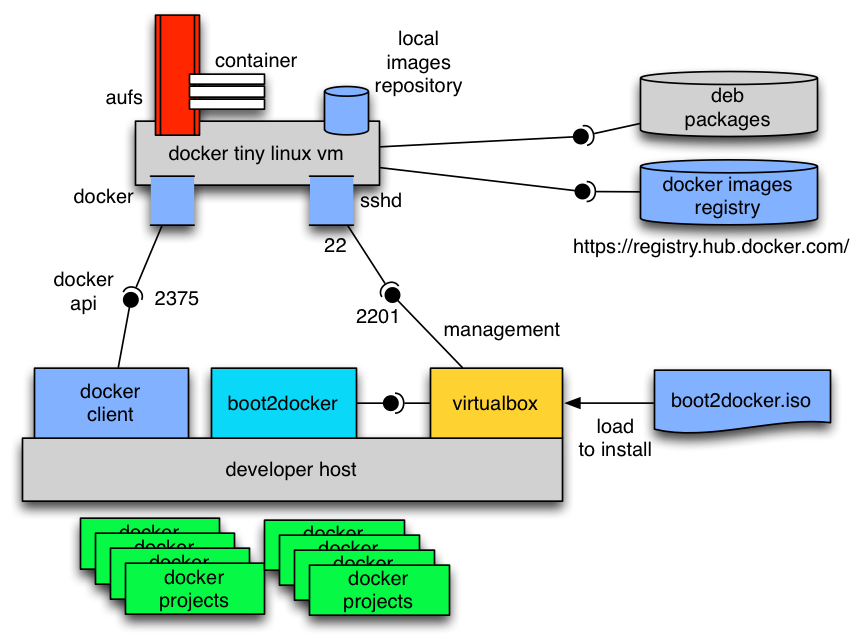
\includegraphics[width=0.9\textwidth]{./images/boot2docker.png}
    \caption{Boot2Docker Architektur sieht dann so aus}
    \label{img:boot2docker}
  \end{center}
\end{figure}
